\chapter{Designing the framework} \label{chapter:design}

Providing the users with a high-level of abstraction is not unheard of in the domain of practical AI platforms. Many software-as-a-service products offer features for hiding the details of machine learning applications. However --- as we saw in Section \ref{section:existing} --- these tend to abstract away the details of both data science and AI-engineering, overall hindering the development process. The design proposed here aims to simplify only the deployment related concepts.

\section{Scope} \label{section:scope}

As highlighted by several case studies in Chapter \ref{chapter:background}, the transition from prototypes to production-ready systems is often named as the source of unexpected struggle. Maybe it is not a coincidence that a significant portion of the SE4ML best practices should be implemented in this phase as well. Unfortunately, it is easy to gloss over them while tackling the underestimated difficulties of this \textit{transition}. Therefore, the aim of GreatAI is to ease this step of the life-cycle, consequently, its scope is limited to the \textit{transition} step.

There have been attempts that at least partially address this issue, however, as we have seen in Chapter \ref{chapter:background}, these have limitations either from the perspective of best practices, or stemming from their difficulty to be adopted. To have the best chance of providing an easy-to-adopt solution, the scope has to be well-defined and limited. Because to understand the API of a library, users first have to understand its aim, surface, and have to become familiar with the problems it solves. Thus, focusing only on the \textit{transition} step seems reasonable. This step is highlighted in Figure \ref{fig:scope}.

\begin{figure}
    \centering
    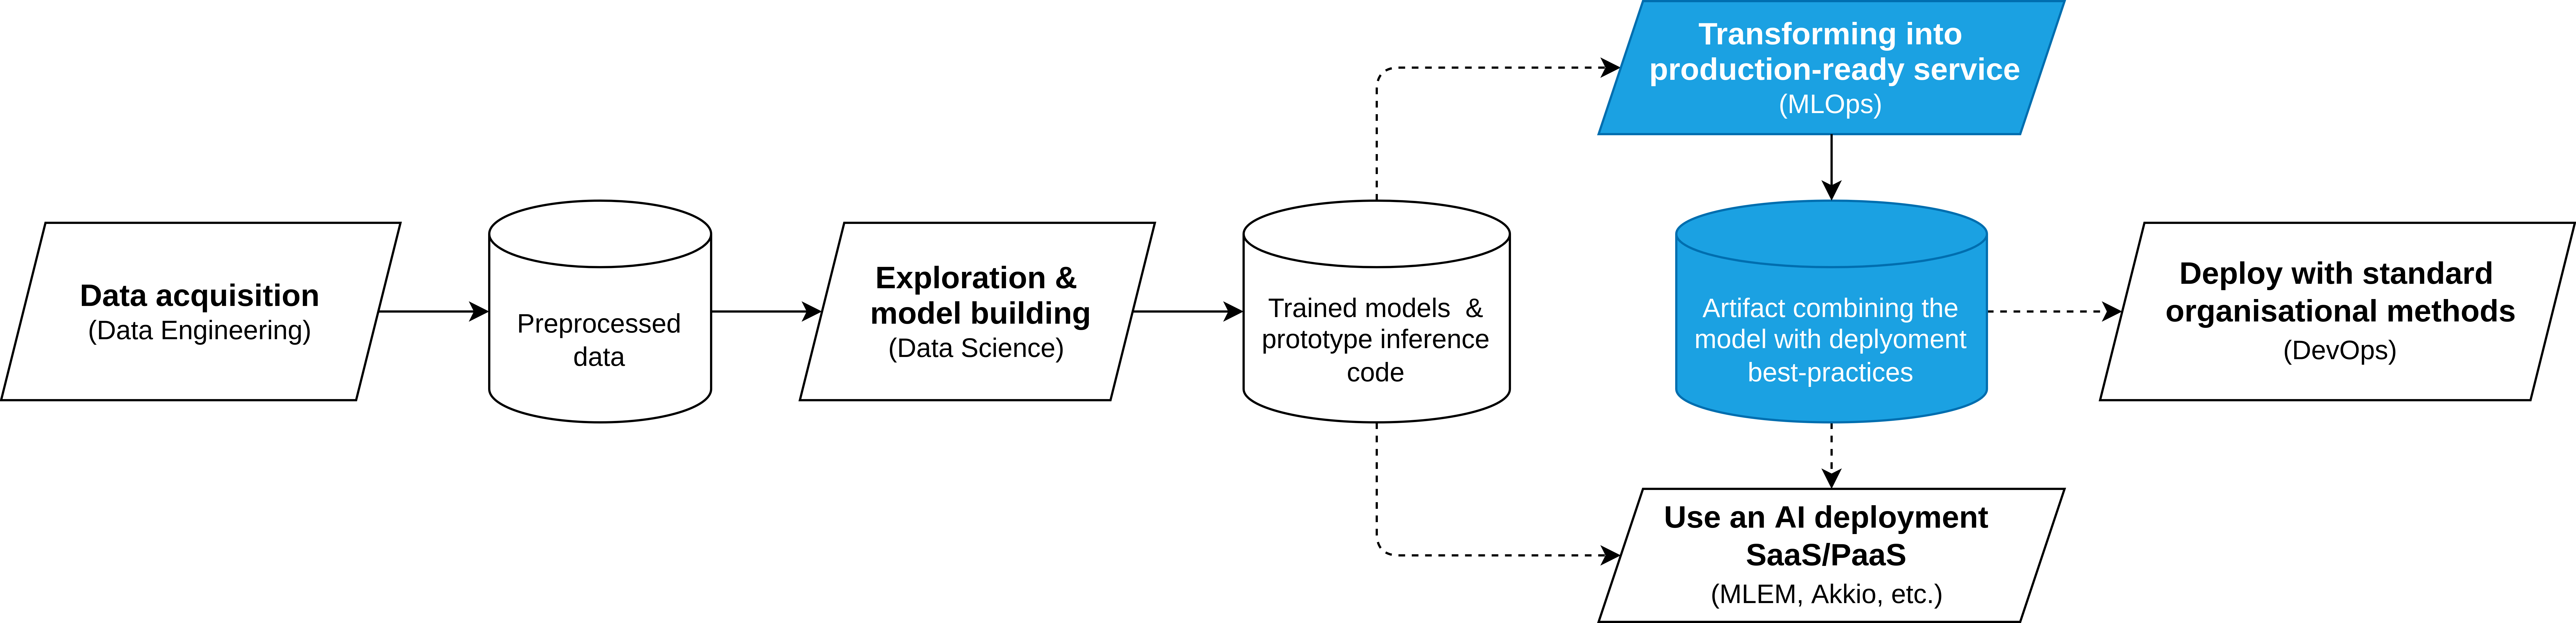
\includegraphics[width=\linewidth]{figures/scope.drawio.png}
    \caption{Usual process steps in the development life-cycle of a data-heavy software solution. The dashed arrows denote optional paths: after a prototype has been completed, there are multiple options for its deployment. The steps with blue background show the scope of GreatAI.}
    \label{fig:scope}
\end{figure}

It is interesting to mention that there is a proliferation\footnote{\href{https://xkcd.com/927/}{xkcd.com/927}} of platform/software as a service (PaaS/SaaS) products for deploying AI\footnote{Such as \href{https://mlem.ai/}{MLEM} or any AutoML SaaS platform, for example, \href{https://www.akkio.com/role/software-engineers}{Akkio} as these often have a one-click deployment feature as well.}. At first, these may look promising, however, they tend to only focus on getting code easily deployed in the cloud: AI best practices are not prioritised in this setup. Nevertheless, in many cases, it may be a suitable option to use such a service and these can also complement GreatAI as illustrated in Figure \ref{fig:scope}. First, the prototype is transformed into a GREAT service and materialised as a common software artifact implementing the best practices. Then, it is either deployed using a deployment SaaS, or by using the organisation's existing software deployment setup.

\section{Design principles}

As implied in Section \ref{section:scope}, the Unix philosophy \cite{ritchie1978unix,salus1994quarter} of software design is followed. Most notably, the design goal that encourages to \textit{write programs that do one thing and do it well.}\footnote{Of course, \textit{write programs to work together} is also very much applicable, since allowing interoperability is one of the core requirements for GreatAI.}. Apart from providing a clear and simple picture of the intended use cases for the library, this is also in line with the main notion of \textit{A Philosophy of Software Design} \cite{ousterhout2018philosophy}: API-s should be narrow and deep. A narrow width refers to having a small exposed surface area, i.e. having a small number of functions and classes in the public API. While depth implies each of them accomplishing an involved, complex goal. 

In a way, the API-s width is the price the users have to pay (the effort required for learning it) to use it, while the depth is analogous to the return they get from it. Having to learn little and being provided by a lot of functionality maximises return on investment, hence, developer experience (DX). The theoretical frameworks presented in \textit{The Programmer's Brain} \cite{hermans2021programmer} provides us with explanations and vocabulary from psychology for arguing about the cognitive aspects of API designs. In the following, two of them will be used for detailing the design principles: cognitive dimensions of code bases (CDCB) which is an extension of the cognitive dimensions of notation (CDN) framework \cite{blackwell2001cognitive}, and linguistic antipatterns \cite{arnaoudova2016linguistic}. The former comes with a set of dimensions which describe different (often competing) cognitive aspects of code that influence one's ability to perform certain tasks with it.

While linguistic antipatterns provide guidelines for improving consistency and decreasing the false sense of consistency when there is none. Also, choosing the right names for identifiers can help activate information stored in the long-term memory which makes it quicker to comprehend and easier to reason about the code \cite{deissenboeck2006concise}. Finding the most accurate and useful names is harder than it first seems. Accuracy and usefulness are already often competing goals. The more precise the name, the longer and therefore less convenient to use \cite{butler2009relating}. In short, good names are key to good API-s; consciously considering the implications of names has to be an integral part of the design process.

Nonetheless, simple API-s come at a high technical cost. The library has to implement these in a way that still allows high-performance in production \cite{kleppmann2017designing} and avoids being tied to specific libraries or technologies. Inspiration for the latter may be gained from the pipelines of Prado et al. \cite{prado2020bonseyes}: they show that more freedom can be achieved with plug-and-play steps and preconfigured defaults. 

Before diving into the concrete issues solved, let us detail the principles that should be used for implementing them in the scope of this framework.

\subsection{Default configuration}

Existing frameworks oftentimes suffer from the entanglement of numerous levels of abstractions. Instead of exposing each implementation detail and encouraging users to interact with most of them, many of these could be abstracted away. Where configuration may be helpful for advanced users, default values can still be chosen automatically while providing an override option where necessary.

For example, tracing the evaluations and the model versions used in a distributed fashion is very much expected of a trustworthy system. Hence, turning this feature on by default but allowing opting-out from it can result in less scaffolding required from the library's user. It also decreases their up-front cognitive load which by definition flattens the learning-curve \cite{hermans2021programmer}. Similar features can be imagined for providing an access API for the algorithms and for giving feedback, marking outliers, etc.

Being \textit{automated} is listed as a requirement but it is imperative to only automate for simplifying and not for hiding decisions. More precisely, guessing must not be a part of automation. For instance --- an otherwise incredibly useful WebGL library --- TWGL.js\footnote{\href{https://twgljs.org/}{twgljs.org}} has a feature for automatically guessing the type of vectors based on their names. If it matches the \texttt{/colou?r/i} pattern, it is treated as a vector with 3 components\footnote{\href{https://github.com/greggman/twgl.js/blob/e3a8d0ed09f7f5cd4be0e4cb5976081c2b5013aa/src/attributes.js\#L139}{\tiny github.com/greggman/twgl.js/blob/e3a8d0ed09f7f5cd4be0e4cb5976081c2b5013aa/src/attributes.js\#L139}}. It is easy to imagine that this can help in certain scenarios, but it does so at the cost of immense confusion when renaming a variable breaks the application. In CDCB, this equates to scoring high on the dimension of \textit{Hidden dependencies} and low on \textit{Visibility}.

Learning from this, any kind of guessing must be avoided for creating a pleasant API. However, this is in conflict with providing defaults for each configuration value. Even if these would be reasonable defaults derived from educated guesses, they are still merely guesses. Nevertheless, if the users are required to specify each configuration option, that leads to considerably more boilerplate code. This verbosity is captured by the \textit{Diffuseness} dimension of CDCB and, of course, should be minimised.

To resolve this conflict, GreatAI should have recommended values instead of defaults. This can mean a context object (as suggested in \cite{ousterhout2018philosophy}), which contains the result of each design decision that has to be made for a service's deployment. If not configured manually, the recommended values are applied, just like defaults. The values chosen for each parameter must be clearly highlighted. Coming from the library's single responsibility, the number of parameters should not be immense, hence, the user can be expected to comprehend them instead of just being overwhelmed and skimming it.

This way, the library attempts to notify its user about the existence of these decisions but does not force them to manually decide. As a result, no initial configuration is needed for starting out with the library (high \textit{Provisionality}, low \textit{Diffuseness}) and the dependencies are not hidden since they are explicitly highlighted.

\subsection{Documentation}

Without a doubt, good documentation is a prerequisite for adoption. Documentation comes in multiple forms: modern integrated development environments (IDEs) tend to show a popup of a function's documentation when requested, at the same time a more comprehensive online documentation and example projects are also still expected. But descriptive error messages can be also viewed as documentation. The library should have quality documentation for all categories.

Once again, we might notice two competing interests: the level-of-detail and the length of the documentation. For example, FastAPI\footnote{\href{https://fastapi.tiangolo.com/async/\#concurrent-burgers}{fastapi.tiangolo.com}}, a popular Python web framework, has extensive descriptions and explanations on all topics related to Python's import system, the HTTP protocol, concurrency, deployment, etc. The actual framework's documentation is sprinkled over these very broad topics. This is certainly helpful for beginners to acquire knowledge from a single place. Nevertheless, this high-level of accessibility actually hinders the process of finding the relevant sections (in CDCB, this shows a trade-off between the support of Searching and Comprehension tasks). My opinion is that linking to external resources about the library's domain are welcome, but the documentation must have a single responsibility: describing the library itself.

A large portion of software documentations is automatically generated from source code. This has the advantage of always keeping it in sync with code changes, however, it might also signal that the API is too large, since it is inconvenient for the developers to document it by hand.

When it comes to example code, showing at least the minimal starter code, and the way of customising it has to be showcased front and centre. It is a well-known observation that developers only read documentation when they are stuck and there might be some merit to this. Making them not get stuck --- by providing a starter code from which they can explore the API using IntelliSense-like solutions --- should be preferred. For example, another widely popular Python web framework, Flask\footnote{\href{https://flask.palletsprojects.com/en/2.1.x/}{flask.palletsprojects.com/en/2.1.x}}, at this time, has 324 uniformly styled links on its landing page. Out of these, only 2 lead to the quick start code. Of course, it is not hidden, but I argue that the DX could be improved by displaying it more prominently.

\subsection{Developer experience}

Subjectively, the key to good DX is consistency and discoverability. To give an example, the MySQL connector's Python implementation\footnote{\href{https://dev.mysql.com/doc/connector-python/en/}{dev.mysql.com/doc/connector-python/en/}} has a cursor object which exposes a \texttt{fetchone} method. Even though this naming scheme is not conventional in Python since it does not follow \href{https://peps.python.org/pep-0008/}{PEP 8}, at least the API is logical: changing \texttt{sql\_cursor.fetchone()} to \texttt{sql\_cursor.fetchall()} returns all items instead of just one. Using good and consistent names is the key to good DX.

Also, Python codebases are rarely strictly object-oriented (OO), they are a mix of functional, data-driven, and OO programming. Consequently, relying on classes for grouping related functions is not always desirable. Therefore, it is even more imperative to name similar functions similarly. This helps discoverability and chunking \cite{hermans2021programmer} which amount to quicker comprehension.

There is one more reason to prefer consistency. Humans have a limited short-term memory (STM) \cite{miller1956magical}. Even though flags as function parameters are frowned upon by some \cite{martin2009clean}, they are useful, especially, when configuring libraries. However, if there is no convention for the default value of a flag, clients have to remember the flag's name and initial value at the same time, quickly overloading their STM. Thus, in the codebase, all defaults must be \texttt{False}. Sometimes, it can result in a \textit{disable} prefix, which turn into a double negation, users shouldn't ever encounter this themselves since the doubly-negated version is the default, thus when overriding it, it is only singly-negated. This approach also implies, that something may be recommended to be turned on by default.
